\documentclass[12pt, a4paper]{article}

\usepackage[utf8]{inputenc}
\usepackage{lmodern}
%\usepackage{fourier}
\usepackage{setspace}
	\singlespacing

\usepackage[frenchb]{babel}
\usepackage{xspace}
\usepackage[margin= 2.5cm]{geometry}
\pagestyle{plain}
\renewcommand{\thefootnote}{\fnsymbol{footnote}}

\usepackage{tikz}
	\usetikzlibrary{shapes}
\usepackage{graphicx}
	\graphicspath{{img/}}

\usepackage{varioref}
	\renewcommand{\reftextbefore}{page précédente}
	\renewcommand{\reftextfacebefore}{page ci-contre}
	\renewcommand{\reftextafter}{page suivante}
	\renewcommand{\reftextfaceafter}{page ci-contre}
	\renewcommand{\reftextcurrent}{}

\usepackage{amsmath, amsfonts}
\everymath{\displaystyle}


\newcommand{\espace}{\vspace{.8cm}}
\newcommand{\pg}{

}

%% REMPLIR
\usepackage[colorlinks=true, allcolors=blue, pdfborder={0 0 0}]{hyperref}
	\hypersetup{
		pdftitle={Arduinnova},
		pdfsubject={Rapport Arduinnova},
		pdfkeywords={Arduinnova, IARISS, rapport},
		pdfauthor={IARISS Team}
	}
\title{Défi Arduinnova}
\newcommand{\authors}{Florent}

%
\begin{document}

\author{
\includegraphics{../_img/iariss_team.png} \\ {\sffamily \href{http://iarissteam.me}{iarissteam.me}}}
\date{\today}

\maketitle{}

{\sffamily Ce rapport a pour but de présenter rapidement la chartre graphique crée pour notre application. Celle-ci utilise un framework CSS(\href{http://twitter.github.com/bootstrap/}{BootStrap Twitter}) qui permet l'utilisation avancée du CSS, du responsive design et le positionnement des éléments;} 

\espace{}
Pour commencer, voici la page d'accueil de notre application : 
\espace{}
\begin{center}
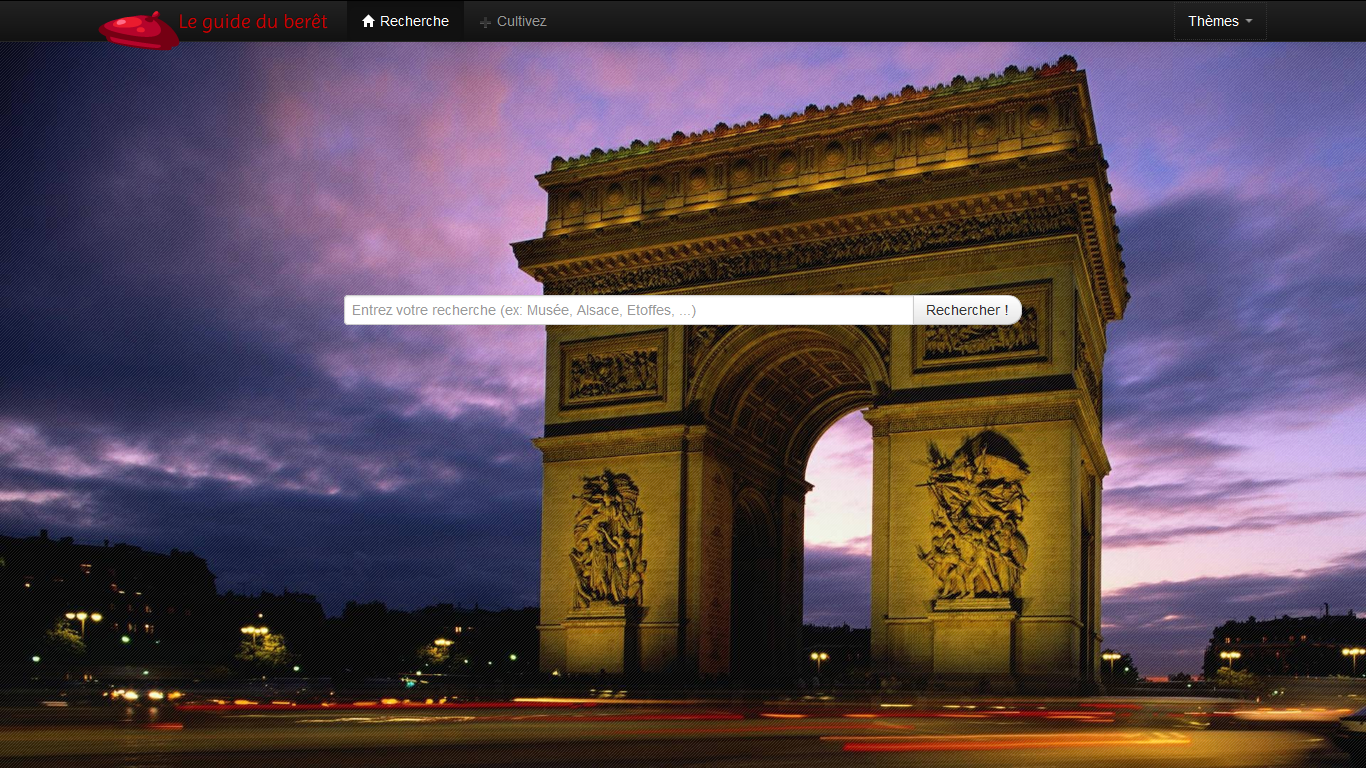
\includegraphics[width=.9\textwidth, keepaspectratio=true]{img/accueil.png}
\end{center}
\espace{}
Nous avons pris le parti de faire un design plutôt sobre et épuré : il est constitué d'une image de fond, par dessus laquel est superposé de très légère rayure. Une barre de navigation est attaché en haut de la fenêtre du navigateur, et une barre de recherche est centrée sur la page. Trois onglets sont disponible dans le menu de navigation : un onglet \og{}Recherche\fg{}, un onglet \og{}Cultivez\fg{} et un onglet \og{}Thèmes\fg{}. Ce dernier permets de changer le thème de la page : en effet, plusieurs thèmes sont disponibles dans notre application. Un changement de thème entraîne le changement de l'image de fond de l'application. Ci-après, exemple : 
\espace{}
\begin{center}
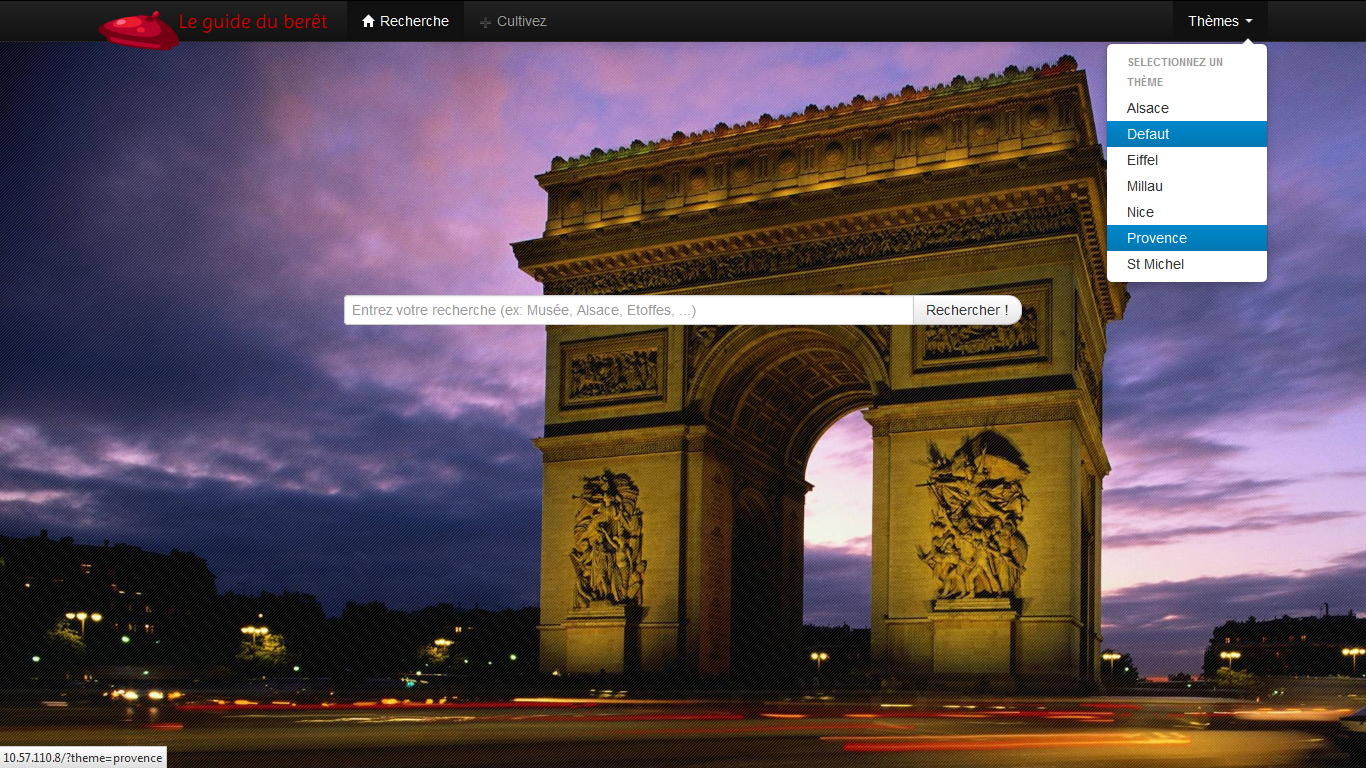
\includegraphics[width=.9\textwidth, keepaspectratio=true]{img/accueil3.png}
\espace{}
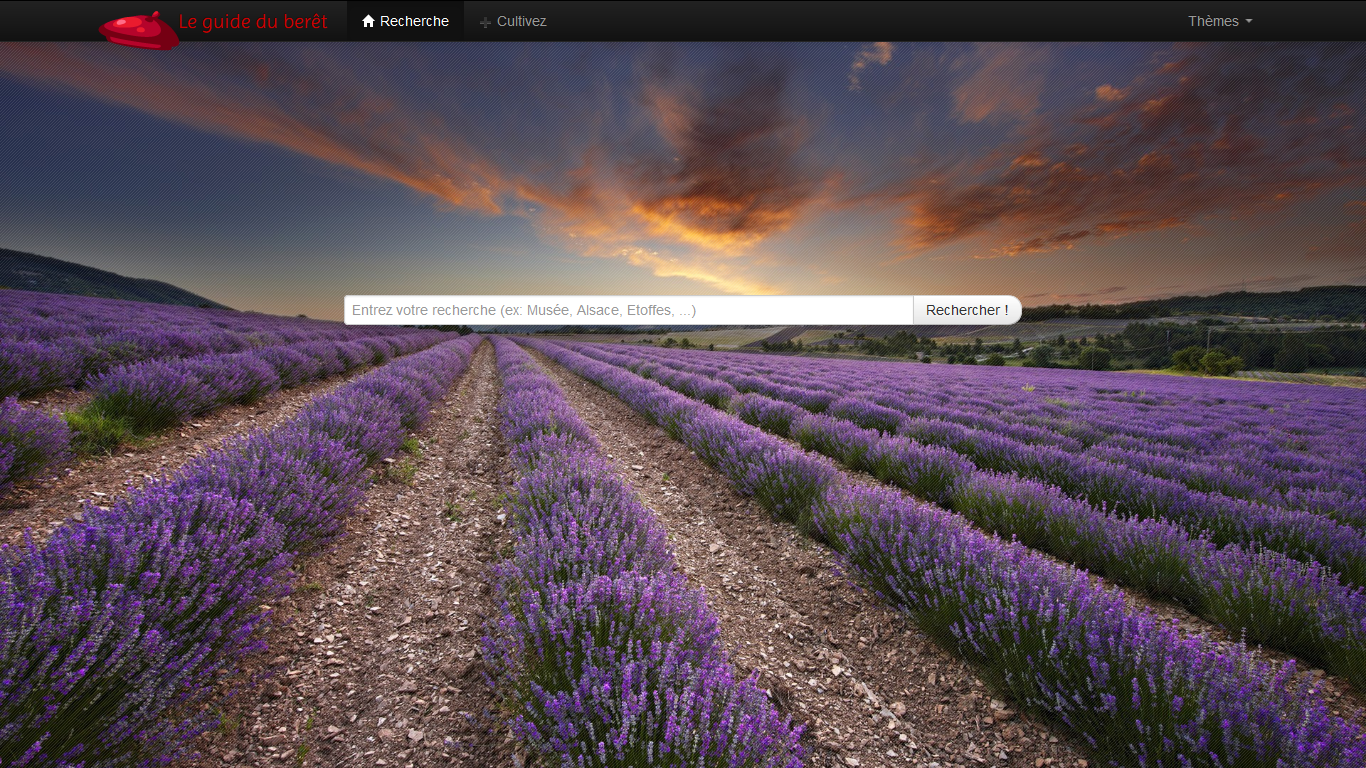
\includegraphics[width=.9\textwidth, keepaspectratio=true]{img/accueil2.png}
\end{center}

\espace{}
Nous allons maintenant nous intéresser à la barre de navigation plus en détails. En plus du menu déroulant permettant de changer le thème du site, nous avons vu qu'il y avait encore deux onglets : \og{}Recherche\fg{} et \og{}Cultivez\fg{}.
Le premier, \og{}Recherche\fg{}, nous affiche la page d'accueil de l'application, à savoir la barre de recherche qui permet à l'utilisateur d'entrer ces mots clés. Le deuxième, \og{}Cultivez\fg{}, permet à l'utilisateur d'ajouter du contenu sur le site : en effet, cette application étant en parti construit sur le principe d'un wiki, il faut que l'utilisateur puisse ajouter son propre contenu.
Le site a également été prévu pour s'adapter aux petites résolutions. En effet, le menu s'adapte automatiquement en fonction de la taille de la fenêtre. Voyons ceci plus en détails avec un exemple : dans les images qui suivent, nous avons volontairement réduit la taille de la fenêtre de notre navigateur.
\espace{}
\begin{center}
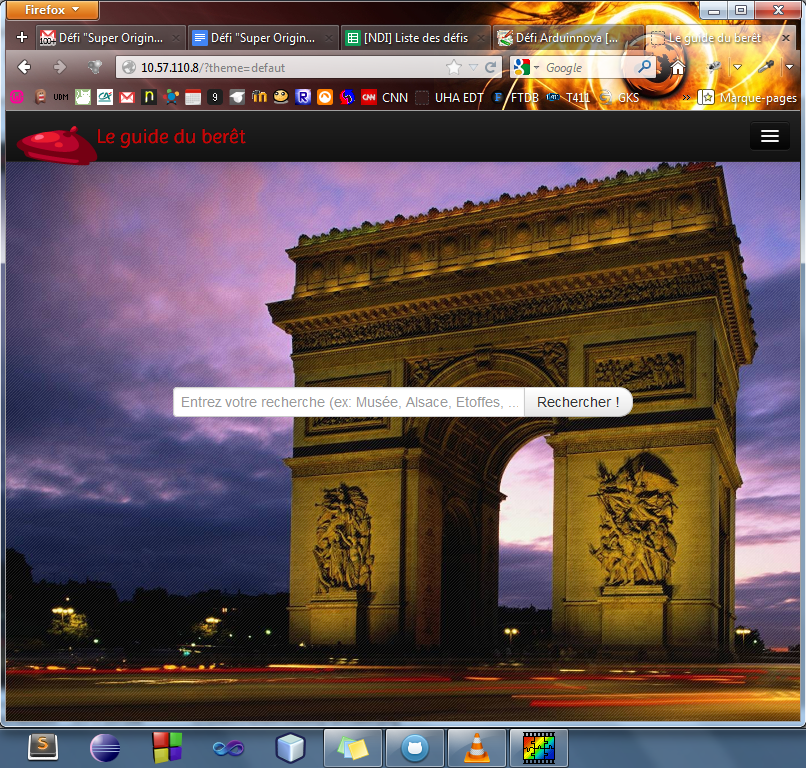
\includegraphics[width=.9\textwidth, keepaspectratio=true]{img/accueil4.png}
\end{center}
\espace{}

On voit déjà que les trois onglets ont disparu et qu'un autre est apparu. Nous allons maintenant cliquer dessus : 

\espace{}
\begin{center}
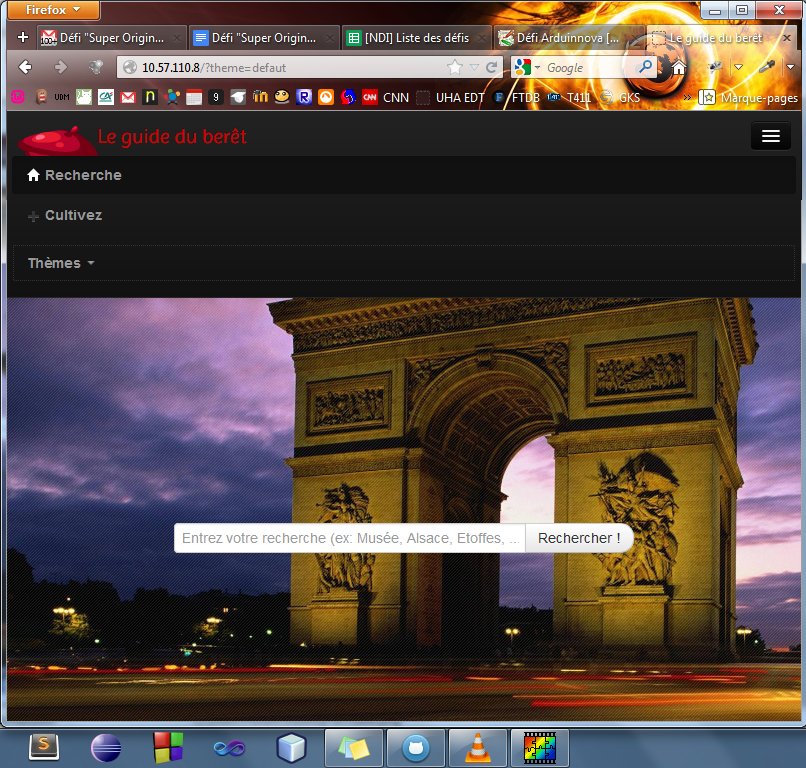
\includegraphics[width=.9\textwidth, keepaspectratio=true]{img/accueil5.png}
\end{center}
\espace{}

On s'aperçoit que l'on retrouve ici nos trois onglets. On peut également continuer à changer le thème, comme précédemment : 

\espace{}
\begin{center}
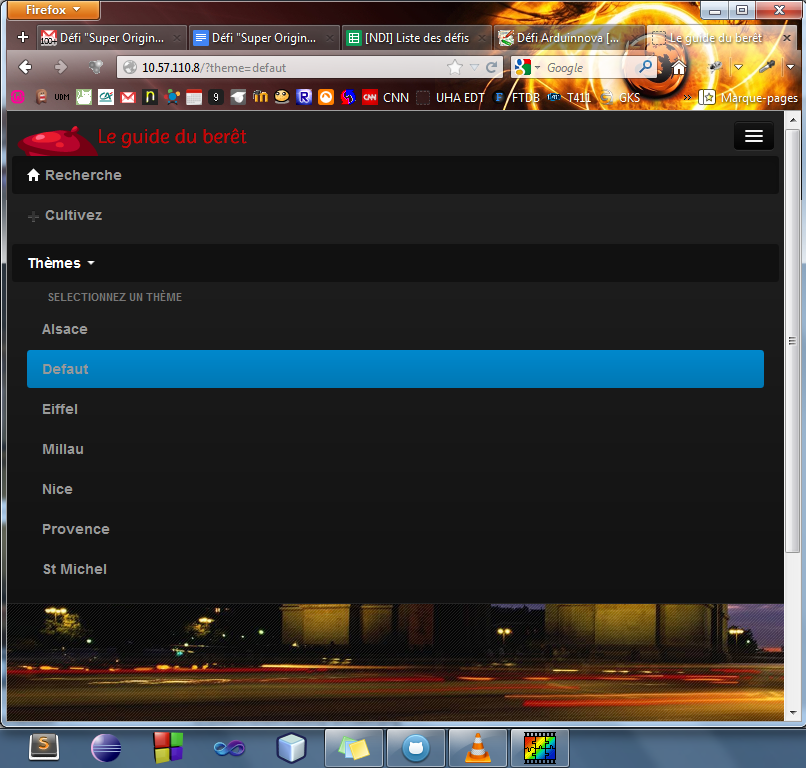
\includegraphics[width=.9\textwidth, keepaspectratio=true]{img/accueil6.png}
\end{center}
\espace{}

En outre, nous avons respecté le thème Alsaco-Canadien demandé par l'un des défis : en effet, à l'utilisation du \href{http://fr.wikipedia.org/wiki/Code_Konami}{code Konami} (haut haut bas bas gauche droite gauche droite B A), un easter egg se déclenchera. De même, à l'utilisation de la chaîne de caractère \og{}je suis un caribou\fg{} dans la page, un autre easter egg se déclenchera.


%\espace{}
%\begin{figure}[h]
%	\begin{center}
%	\end{center}
%	\caption{\label{fig-} Légende}
%\end{figure}

\espace\vfill{}
Ce document a été rédigé en \LaTeX{} par \authors{} pour IarissTeam avec quelques tasses de café et beaucoup de bonne humeur.

Contactez-nous à \href{mailto:nuitinfo@iariss.com}{nuitinfo@iariss.com} pour tout renseignement supplémentaire !

\end{document}